\documentclass{article}
\usepackage{scrextend}
\usepackage{xcolor}
\usepackage[spanish, english]{babel} 
\usepackage[spanish]{babel}
\usepackage[dvips,a3paper,centering,margin=2cm]{geometry}
\usepackage{multicol}
\usepackage[utf8]{inputenc}
\usepackage{lipsum}
\usepackage{color}
\definecolor{rb}{rgb}{0.025,0.5,0.9} 
\usepackage{graphicx}  
\pagestyle{empty}
\def\to{\rightarrow}
\begin{document}
\vspace*{-2cm}
\changefontsizes{14pt}
\begin{minipage}{0.2\linewidth}
\vspace*{-0.15cm}

\includegraphics[scale=0.18]{images/CCA.png}
\end{minipage}
\vspace*{-0.4cm}
\begin{minipage}{0.6\linewidth}
\changefontsizes{19pt}
\vspace*{0.7cm}
\begin{center}
\textbf{Modelización de la irradiancia solar UV-VIS-NIR* en el área metropolitana de Monterrey, México}\\
\end{center}
\vspace{-1.4cm}
\begin{center}
\changefontsizes{12pt}{
Gamaliel López-Padilla$^1$, Adriana Ipiña$^{2,3}$\\
1. Facultad de Ciencias Físico-Matemáticas,UANL
2. Centro de Ciencias de la Atmósfera, UNAM
3. Instituto de Física Rosario, CONICET-UNR}
\end{center}
\end{minipage}
\begin{minipage}{0.2\linewidth}
\hspace*{1.2cm}

\includegraphics[scale=0.30]{images/fcfm.png}
\end{minipage}
\vspace*{1cm}
\textcolor{rb}{\hrule}
\begin{multicols}{2}
\changefontsizes{15pt}
\vspace*{-1cm}
\begin{center}
\large \textbf{ \textcolor{rb}{Introducción}}
\end{center}
\vspace*{-0.13cm}
La radiación solar puede ser medida in situ o calculada con modelos de transferencia radiativa. Determinar la irradiancia solar nos permite conocer su intensidad, así como caracterizar estos factores que influyen en su atenuación. Presentamos un avance del análisis de la irradiancia UV e irradiancia global estimadas con el modelo TUV (Tropospheric Ultraviolet and Visible Radiation Model) y medidas por el SIMA (Sistema Integral de Monitoreo Ambiental) para la cuidad de Monterrey y su área metropolitana.
\vspace*{-0.2cm}
\begin{center}
\large \textbf{\textcolor{rb}{Materiales y Métodos}}
\end{center}
Se realizaron mediciones de irradiancia solar con dos radiómetros UVA+UVB y UVB Solarmeter, tomándose de referencia para estimar el AOD$_{550nm}$, ejecutando el modelo TUV hasta alcanzar los valores medidos. Los parametros de entrada son: las coordenadas geográficas, reflectividad del suelo, hora, fecha y las columnas totales de O$_3$ y NO$_2$ (medidas por OMI-Aura los dias considerados) entre otros. 
Este criterio se aplicó también para obtener la irradiancia espectral en los rangos UV-VIS-NIR* en dos estaciones del área metropolitana de Monterrey. Se calcularon las irradiancias globales (Eglob en W/m$^2$ ) en el rango de 400nm a 1000nm, comparándolas con las mediciones del SIMA. Se eligieron dias de cielo despejado en verano e inverno para las estaciones Noroeste (San Nicolas) y Noroeste (San Bernabé).
\vspace*{-0.3cm}
\begin{center}
\large \textbf{\textcolor{rb}{Resultados}}
\end{center}
Los resultados del modelo indican que, para esta época del año, al mediodia solar y cielo despejado, la irradiancia UVA+UVB y UVB es alrededor de 55 W/m$^2$ , y 4 W/m$^2$ respectivamente, mientras que el indice UV máximo diario es 10. Del modelo TUV se derivaron los espectros solares en el intervalo 280-1000nm a lo largo de las horas del día, éstos fueron procesados para determinar la irradiancia en el rango VIS-NIR*. Para esto se escribió un código que calcula la integral desde 400nm a 1000nm y así obtener la irradiancia solar en una hora determinada\\
\vspace*{-0.7cm}
\begin{center}
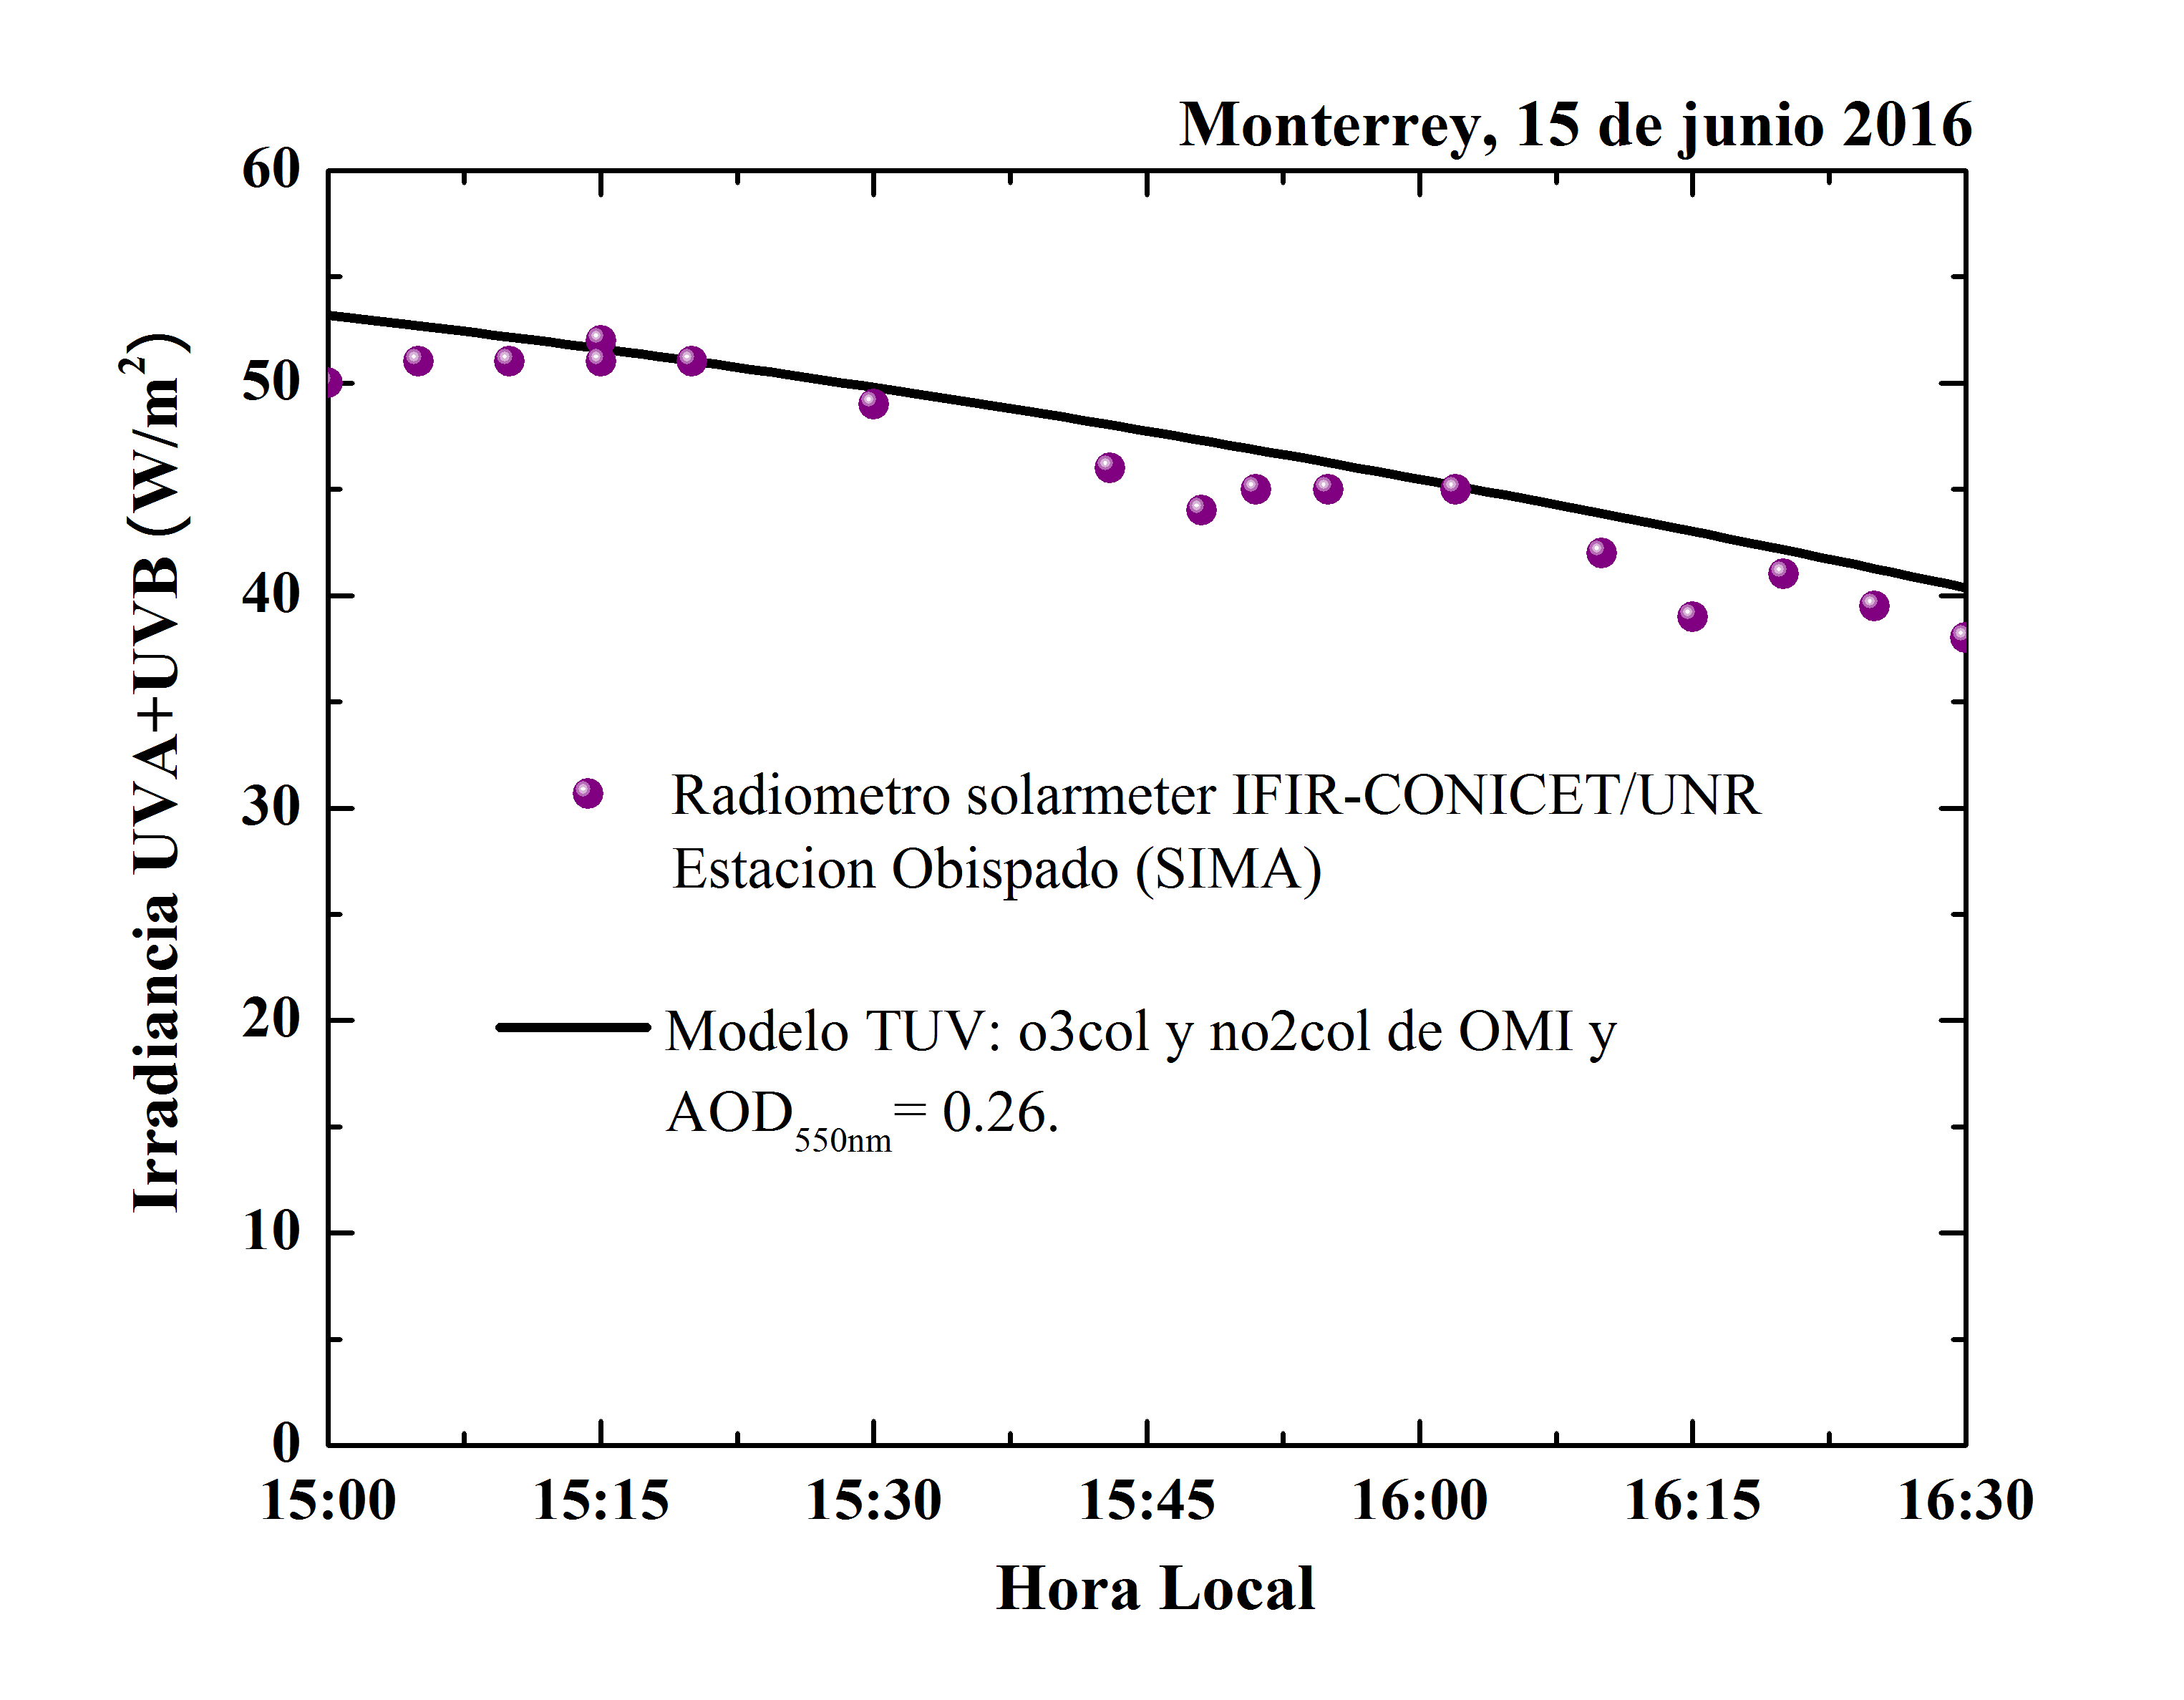
\includegraphics[width=0.65\linewidth]{images/sima2.jpg}\\
\changefontsizes{12pt}
Figura 1: Modelo TUV ajustado para la irradiancia UVA+UVB medida con radiómetro Solameter en la estación Centro
\end{center}
\begin{center}
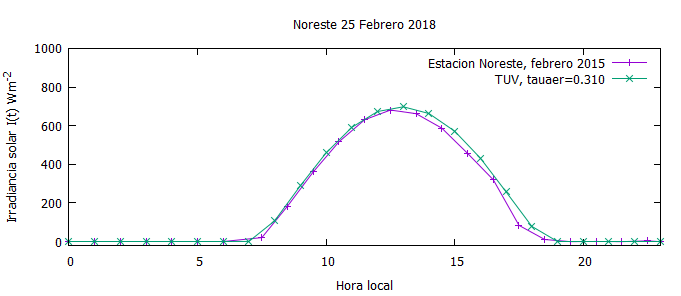
\includegraphics[scale=0.44]{images/nef.png}\\
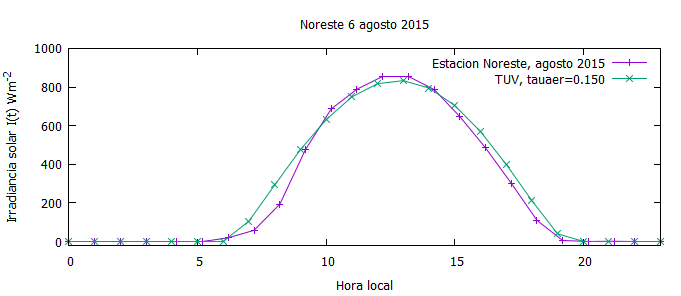
\includegraphics[scale=0.44]{images/neg.png}\\
%\vspace*{-0.5cm
\changefontsizes{12pt}
Figura 2: Irradiancia solar correspondiente a la estación Noreste\\
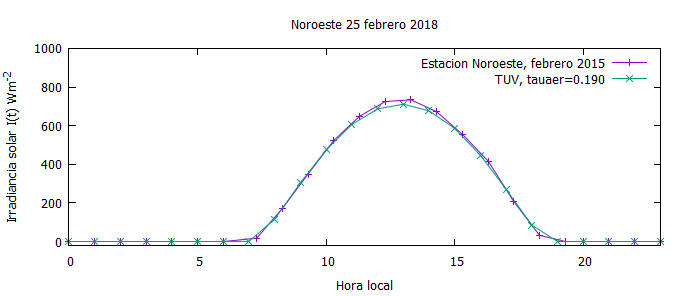
\includegraphics[scale=0.44]{images/nof.png}\\
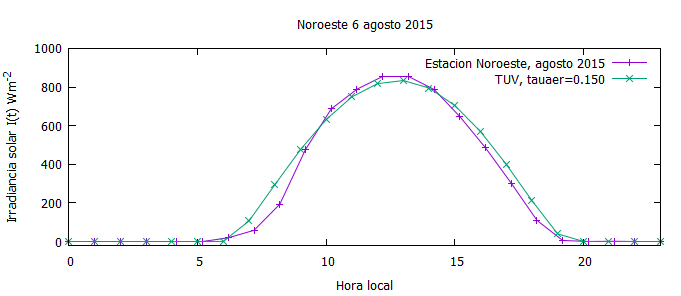
\includegraphics[scale=0.44]{images/nag.png}\\
\changefontsizes{12pt}
Figura 3: Irradiancia solar correspondiente a la estación Noroeste\\
\end{center}
\vspace*{-0.62cm}
\begin{center}
\large \textbf{\textcolor{rb}{Conclusiones}}
\end{center}
\vspace*{-0.3cm}
Las diferencias relativas al mediodia solar entre el modelo y la medición de irradiancia global fueron: 2.3\% y 0.5\% en agosto, mientras que en febrero 2.4\% y 3.1\% para las estaciones Noreste y Noroeste respectivamente. Los valores de AOD$_{550nm}$ encontrados fueron menores en agosto, pudiera ser por la precipitación antecedida a los días de cielo claro utilizados en la comparación. Las diferencias al inicio y al final del día probablemente se deban a la variación del AOD$_{550nm}$, el O$_3$ troposférico y el NO$_2$ en función del tiempo, ya que afectan en mayor medida. Este análisis se extenderá para conocer la proporción de afectación de cada uno.
\begin{center}
\large \textbf{\textcolor{rb}{Referencias}}
\end{center}
\begin{enumerate}
\changefontsizes{12pt}
\vspace*{-0.4cm}
\item TUV model from Madronich \\https://www2.acom.ucar.edu/modeling/tropospheric-ultraviolet-and-visible-tuv-radiation-model
\vspace*{-0.3cm}
\item Ipiña A, Salum GM, Crinó E, Piacentino RD. Satelite and ground detection of very dense smoke clouds produced on the islands of the Paraná river delta that affected a large region in Central Argentina, ASR. 49, 966-977 (2012)
\vspace*{-0.3cm}
\end{enumerate}
%\begin{center}
%\large \textbf{\textcolor{rb}{Agradecimientos}}
%\end{center}
%\vspace*{-0.1cm}
%A la REDCAM Conacyt por el apoyo brindado a G.G.L y a DGAPA (UNAM) por la beca otorgada a A.I.
\end{multicols}
\end{document}